\section{Implementation Details of \method}
\label{app:implementation}

\subsection{Attention Mask Design}
\begin{figure}[!ht]
    \centering
    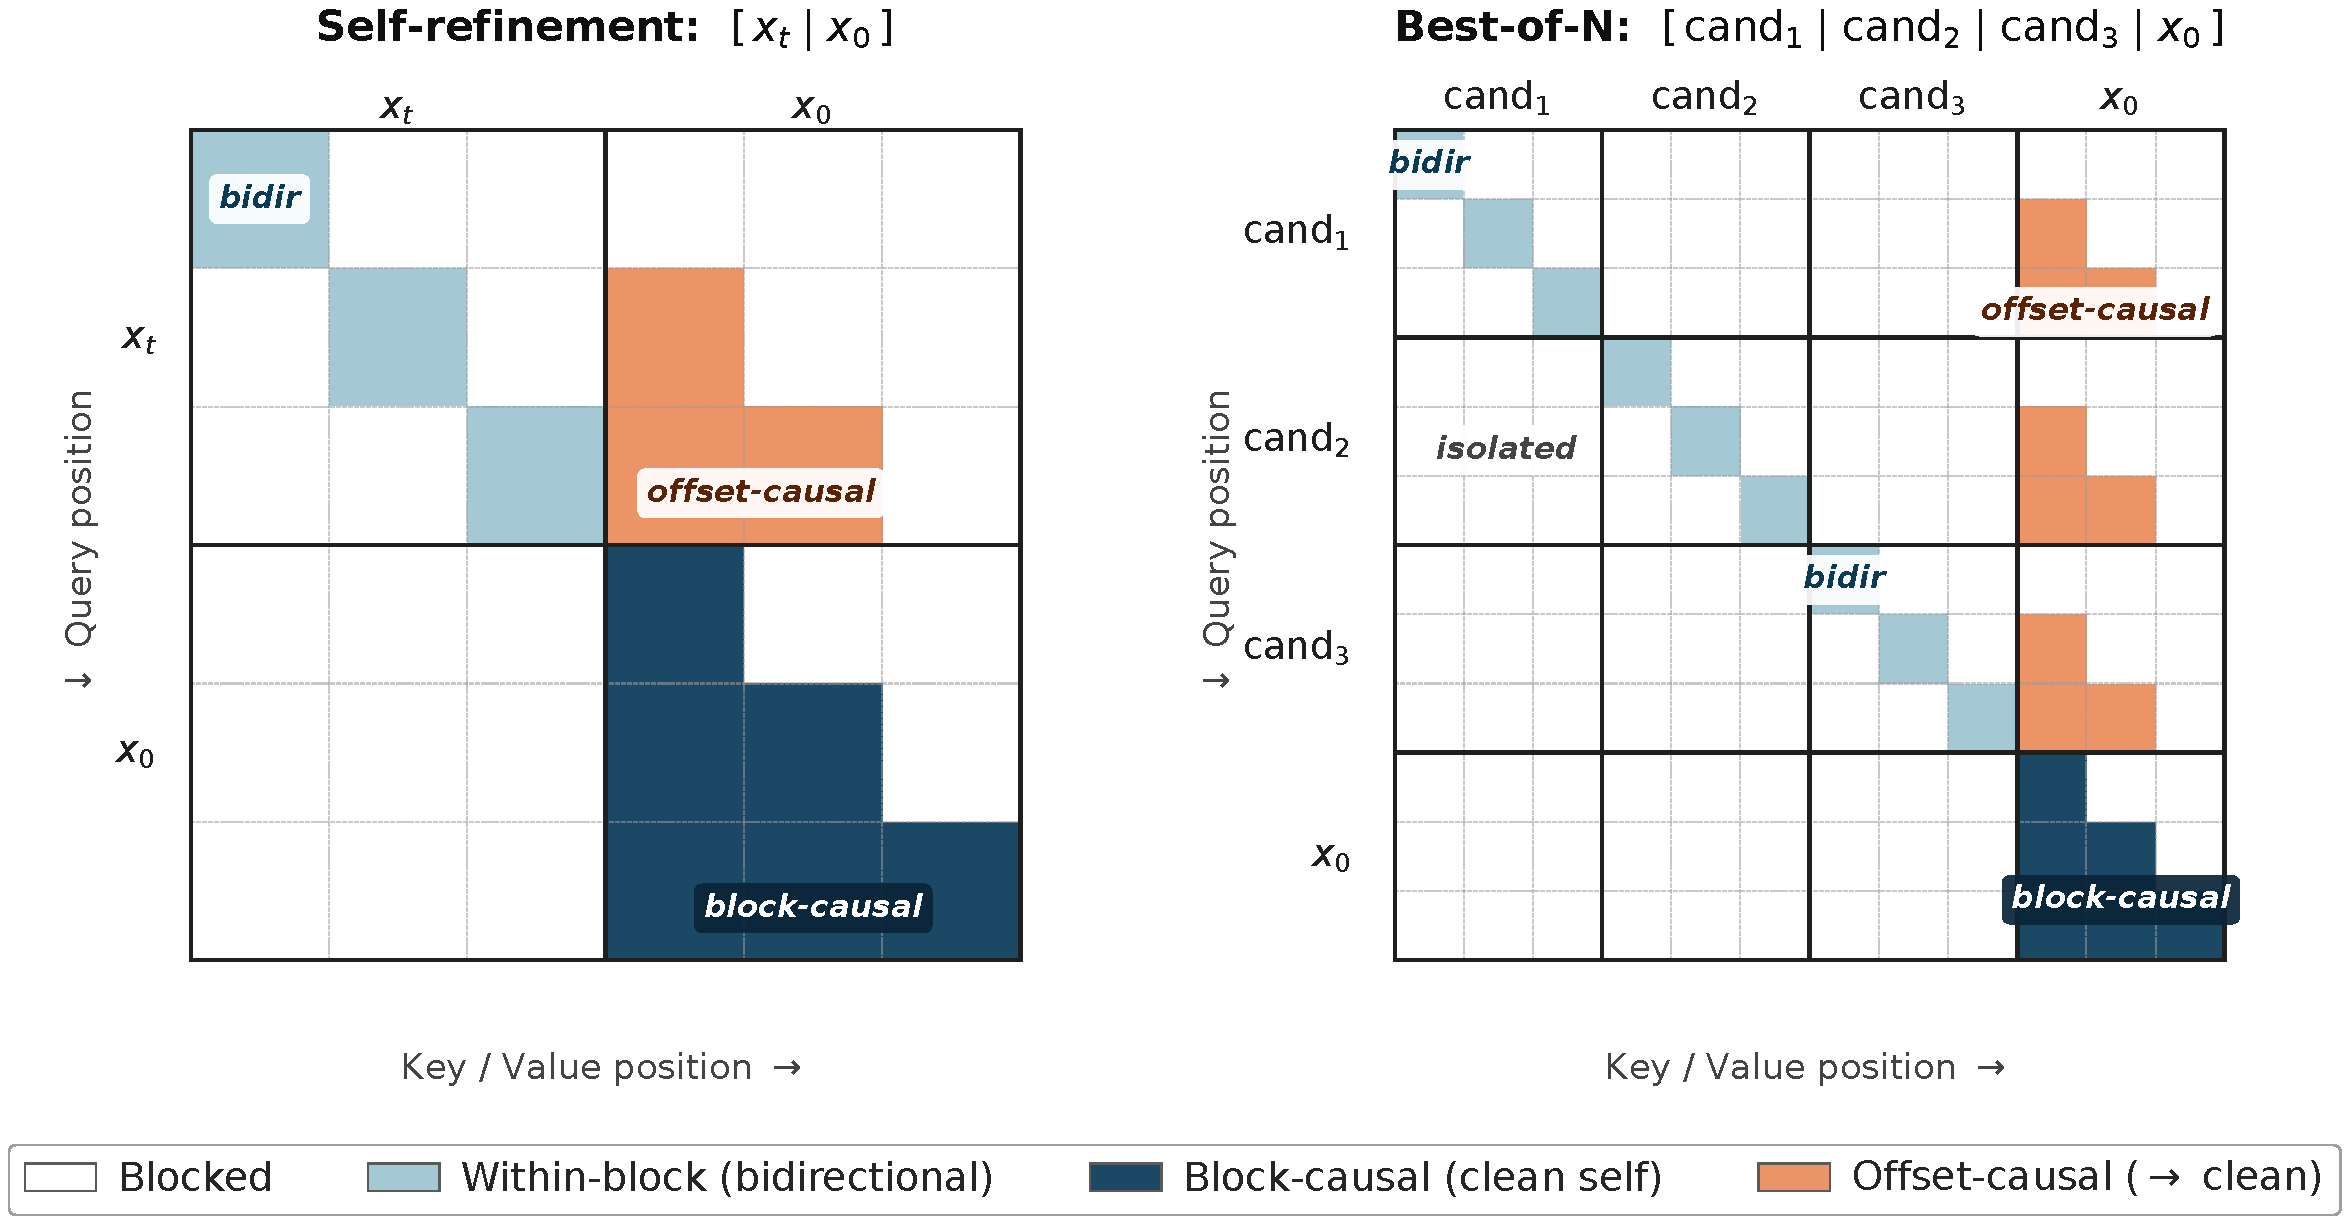
\includegraphics[width=\linewidth]{figures/attn_mask_design.pdf}
    \caption{Attention mask design for \method's Self-refinement and Best-of-N forwards.}
    \label{fig:attn-mask-design}
\end{figure}

Figure~\ref{fig:attn-mask-design} illustrates the attention masks used for self-refinement and Best-of-$N$ refinement. We adopt a similar mask design for self-refinement following ~\citep{block_diffusion, sdar, llada20}.
In self-refinement, the input is organized as $[\dv_t \mid \dv_0]$. 
The refinement segment $\dv_t$ uses bidirectional attention within each block, allowing all positions in the current block to be jointly denoised, while the clean segment $\dv_0$ uses block-causal attention. 
In addition, refinement block $j$ can attend only to clean blocks $0,\ldots,j-1$, ensuring that the model conditions on committed prefix tokens without seeing the clean version of the block being refined. 
For Best-of-$N$ refinement, the input is organized as $[\mathrm{cand}_1\mid\cdots\mid\mathrm{cand}_N\mid\dv_0]$ and follows the same within-block bidirectional and offset-causal rules, but different candidate segments are mutually isolated. 
This isolation ensures that each candidate is scored only from its own tokens and the shared clean prefix, preventing the scorer from exploiting interactions among candidates. 
The bidirectional within-block attention enables global refinement and scoring within each block, while the block-causal structure preserves efficient left-to-right block generation. 


\begin{wrapfigure}{r}{0.4\textwidth}
    \vspace{-4.0em}
    \centering
    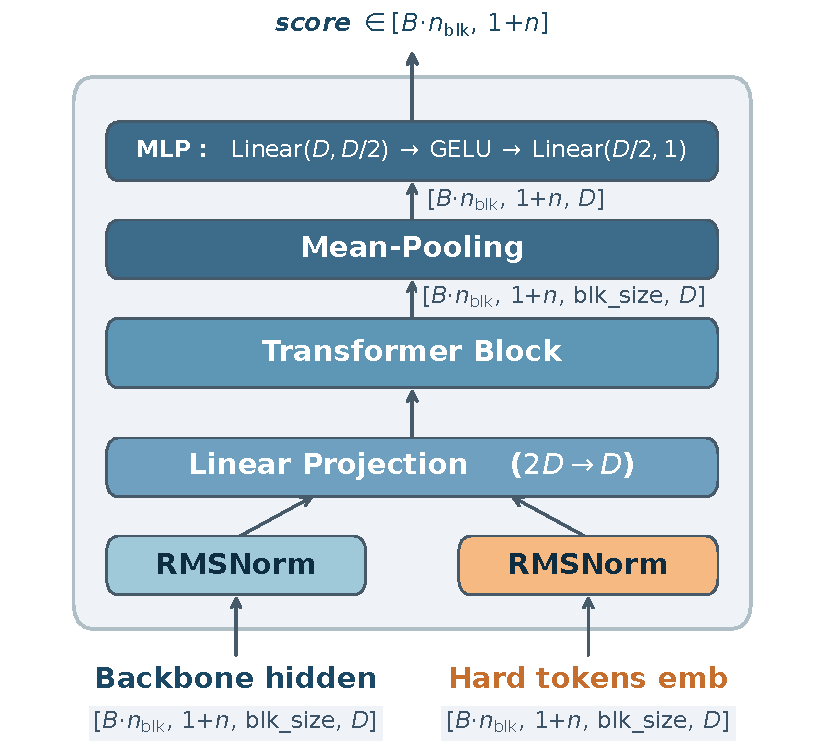
\includegraphics[width=0.98\linewidth]{figures/scorer_arch.pdf}
    \caption{
    Best-of-$N$ scorer head with soft--hard fusion.
    }
    \label{fig:scorer-arch}
    \vspace{-1.0em}
\end{wrapfigure}

\subsection{Best-of-$N$ Scorer Architecture}
\label{app:scorer_arch}

The Best-of-$N$ variant of \method uses a lightweight scorer head to rank block-level candidate refinements. 
As shown in Fig.~\ref{fig:scorer-arch}, the scorer shares the self-refinement backbone, which is mostly frozen during scorer training, and predicts one scalar score for each candidate slot. 
Given $n$ candidate refinements and one clean positive slot, the scorer processes $(1+n)$ slots per block and is trained with the Best-of-$N$ objective, which treats the clean $x_0$ slot as the positive.

For each candidate, the scorer uses two complementary input channels. 
The soft channel is the frozen backbone hidden state $H$, which captures contextual compatibility under the blockwise attention pattern. 
The hard channel is the embedding of the candidate's discrete argmax tokens which preserves token-level identity information that may be weakened by the soft embedding. 
Inspired by the feature fusion adopted in multi-token prediction~(MTP) module in DeepSeek-V3~\citep{deepseek-v3}, the two channels are separately normalized and fused through a linear projection:
\[
    Z
    =
    W_{\mathrm{fuse}}
    \left[
        \mathrm{RMSNorm}(H)
        \,;\,
        \mathrm{RMSNorm}\rbr{E(\arg\max c)}
    \right].
\]
The fused representation is processed by a lightweight Qwen3-style Transformer block~\citep{qwen3}, masked mean pooling, and a two-layer MLP:
\begin{align*}
    s(c)
    &=
    \mathrm{MLP}
    \left(
        \mathrm{MeanPool}
        \rbr{
            \mathrm{TransformerBlock}(Z)
        }
    \right),
    \\
    \mathrm{MLP}
    &=
    \mathrm{Linear}(D,D/2)
    \rightarrow
    \mathrm{GELU}
    \rightarrow
    \mathrm{Linear}(D/2,1).
\end{align*}
The resulting $(1+n)$ scores are normalized with a softmax under the Best-of-$N$ objective. 
Because the scorer reuses the frozen proposer backbone and only adds a small head over pooled block representations, Best-of-$N$ selection remains efficient during both training and inference.



\subsection{Soft Prediction Embedding}
To represent sampler-induced drafts during recursive refinement, we adopt a soft prediction embedding from \citep{dmax}, rather than feeding back only hard argmax tokens. 
Let $h_i^{(t)}$ be the logits at position $i$ after refinement step $t$, and let
\begin{equation*}
    \hat{x}_i^{(t)}
    =
    \arg\max_{v\in\Vcal} h_{i,v}^{(t)}
\end{equation*}
denote the selected token. 
We construct the next-step input embedding as
\begin{equation}
    e_i^{(t+1)}
    =
    \alpha_i^{(t)}
    E\rbr{\hat{x}_i^{(t)}}
    +
    \rbr{1-\alpha_i^{(t)}}
    E\rbr{\blanktoken},
    \qquad
    \alpha_i^{(t)}
    =
    \mathrm{softmax}\rbr{h_i^{(t)}}_{\hat{x}_i^{(t)}},
    \label{eq:soft_prediction_embedding}
\end{equation}
where $E$ is the token embedding table and $\alpha_i^{(t)}$ is the model probability of the selected token. 
Thus, high-confidence selected tokens are represented close to their hard token embeddings, while uncertain predictions remain close to the mask embedding and can be further refined. 
This confidence-weighted interpolation is related to recent smoothing and trace-based decoding techniques for diffusion language models~\citep{smoothie,credit-decoding}. 
Unlike methods that apply such smoothing only during inference, \method uses the same soft prediction embedding during both training and inference, reducing the train--inference mismatch of intermediate drafts and improving refinement stability.

\begin{algorithm}[!htbp]
    \SetAlgoLined
    \DontPrintSemicolon
    \SetNoFillComment
    \SetNlSkip{0.4em}
    \LinesNotNumbered
    \linespread{.86}\selectfont
    \caption{\method Training}
    \label{alg:training}
    \SetKwInput{KwIn}{Input}
    \SetKwInput{KwOut}{Output}

    \KwIn{
    Training corpus $\Dcal$; refinement backbone $K_{\theta}$; optional scorer $\scorer$; \\
    maximum refinements $K_{\max}$; Best-of-$N$ width $n$; blockwise attention mask $\Mcal_{\mathrm{block}}$ from Fig.~\ref{fig:attn-mask-design}.
    }
    \KwOut{Trained self-refinement model $K_{\theta}$ and optional Best-of-$N$ scorer $\scorer$.}

    \tcc{Stage I: train sampler-induced self-refinement}
    Initialize $K_{\theta}$ from the base language model\;
    \For{training step}{
        Sample clean sequence $\dv_0\sim\Dcal$ and sample $K\le K_{\max}$\;
        Initialize draft $\dv_K\leftarrow[\blanktoken]$ for the current block\;
        \For{$r=K,\ldots,1$}{
            Form training input $\ub_r\leftarrow[\,\dv_r;\dv_0\,]$\;
            Run $K_{\theta}$ on $\ub_r$ with blockwise attention mask $\Mcal_{\mathrm{block}}$\;
            \eIf{$r>1$}{
                Update draft $\dv_{r-1}$ from the prediction with no gradient\;
                $\dv_{r-1}\leftarrow\mathrm{stopgrad}\rbr{\dv_{r-1}}$\;
            }{
                Update $\theta$ by minimizing the self-refinement loss in Eq.~\eqref{eq:self_refine_loss}\;
            }
        }
    }

\tcc{Stage II: train Best-of-$N$ scorer, if used}
\If{Best-of-$N$ refinement is enabled}{
    Freeze the refinement backbone $K_{\theta}$\;
    \For{training step}{
        Sample clean positive $\dv^{+}\sim\Dcal$ and sample $K\le K_{\max}$\;
        Generate $n$ candidate refinements $\{\dv_i^{-}\}_{i=1}^{n}$ by running the self-refinement sampler with frozen $K_{\theta}$\;
        Concatenate positive and candidates into one BoN input 
        $\ub_{\mathrm{bon}}\leftarrow[\,\dv^{+};\dv_1^{-};\cdots;\dv_n^{-}\,]$\;
        Run frozen $K_{\theta}$ on $\ub_{\mathrm{bon}}$ with BoN attention mask $\Mcal_{\mathrm{BoN}}$, which isolates candidate slots\;
        Score the $(1+n)$ slots with $\scorer$\;
        Update $\phi$ with the Best-of-$N$ objective in Eq.~\eqref{eq:bon_loss}\;
    }
}
\end{algorithm}

\subsection{Pseudocode for Training and Inference}
\label{app:pseudocode}

We provide pseudocode for the main training and decoding procedures of \method. 
Algorithm~\ref{alg:training} summarizes the two-stage training pipeline, including sampler-induced self-refinement training and optional Best-of-$N$ scorer training. 
Algorithm~\ref{alg:self-refine-infer} describes self-refinement decoding for a single block, where the model iteratively updates a draft and commits high-confidence tokens. 
Algorithm~\ref{alg:bon-one-block} extends this procedure with Best-of-$N$ candidate selection, and Algorithm~\ref{alg:beam-sampling} details the marginal-cost beam sampler used to construct diverse candidate blocks efficiently.




\begin{algorithm}[!htbp]
    \SetAlgoLined
    \DontPrintSemicolon
    \SetNoFillComment
    \LinesNotNumbered
    \linespread{.86}\selectfont
    \caption{Self-Refinement Decoding for One Block}
    \label{alg:self-refine-infer}
    \SetKwInput{KwIn}{Input}
    \SetKwInput{KwOut}{Output}

    \KwIn{Refinement backbone $K_{\theta}$; committed prefix $x_{\mathrm{pre}}$; block size $B$; refinement budget $K$; confidence threshold $\eta$.}
    \KwOut{Decoded block $\hat c\in\Vcal^B$.}

    Initialize $\hat c \leftarrow [\blanktoken]^B$ and commitment mask $m\leftarrow[0]^B$\;
    Initialize $p \leftarrow \mathrm{Uniform}(\Vcal)^B$\;

    \For{$k=1,\ldots,K$}{
        \eIf{$k=1$}{
            Form input $\ub\leftarrow[\,\hat c;x_{\mathrm{pre}}\,]$ using hard blank tokens\;
        }{
            Build soft input embeddings $e\leftarrow\textsc{SoftEmbed}(\hat c,p,m)$ using Eq.~\eqref{eq:soft_prediction_embedding}\;
            Form input $\ub\leftarrow[\,e;x_{\mathrm{pre}}\,]$\;
        }

        Compute $p \leftarrow \mathrm{softmax}\rbr{K_{\theta}(\ub;\Mcal_{\mathrm{block}})}_{1:B}$\;
        Set $\tilde c_i \leftarrow \arg\max_{v\in\Vcal} p_{i,v}$ and $\alpha_i\leftarrow p_{i,\tilde c_i}$ for all $i$\;

        Reset $m\leftarrow[0]^B$\;
        \tcc{Early commitment.}
        \For{$i=1,\ldots,B$}{
            \eIf{$\alpha_i\ge\eta$}{
                $\hat c_i\leftarrow\tilde c_i$ and $m_i\leftarrow1$\;
            }{
                \textbf{break}\;
            }
        }

        \tcc{Early stop if all positions in the block are committed.}
        \If{$\forall i,\ m_i=1$}{
            \textbf{break}\;
        }
    }

    \tcc{If the iteration budget is exhausted, force-commit remaining positions.}
    \For{each $i$ with $m_i=0$}{
        $\hat c_i\leftarrow \arg\max_{v\in\Vcal}p_{i,v}$\;
    }

    \Return{$\hat c$}\;
\end{algorithm}

\begin{algorithm}[!htpb]
    \SetAlgoLined
    \DontPrintSemicolon
    \SetNoFillComment
    \LinesNotNumbered
    \linespread{.86}\selectfont
    \caption{Best-of-$N$ Refinement Decoding for One Block}
    \label{alg:bon-one-block}
    \SetKwInput{KwIn}{Input}
    \SetKwInput{KwOut}{Output}

    \KwIn{
    Refinement backbone $K_{\theta}$; scorer $\scorer$; committed prefix $x_{\mathrm{pre}}$; \\
    block size $B$; refinement budget $K$; width $n$; commitment threshold $\eta$; scorer weight $\tau$.
    }
    \KwOut{Decoded block $\hat c\in\Vcal^B$.}

    Initialize draft $\hat c\leftarrow[\blanktoken]^B$, commitment mask $m\leftarrow[0]^B$, and $p\leftarrow\mathrm{Uniform}(\Vcal)^B$\;

    \For{$k=1,\ldots,K$}{
        \tcc{Generate $n$ candidate drafts from the current state.}
        Generate candidate drafts $\{\hat c_i\}_{i=1}^{n}$ from $\hat c$ using marginal-cost beam sampling or stochastic candidate sampling\;
        Compute proposal scores $\ell_i\leftarrow\log q_{\theta}\rbr{\hat c_i\mid \hat c,x_{\mathrm{pre}}}$ for $i=1,\ldots,n$\;

        \tcc{One packed BoN forward gives both refinement predictions and scorer values.}
        Form BoN input 
        $\ub_{\mathrm{bon}}\leftarrow[\,\hat c_1;\hat c_2;\cdots;\hat c_n;x_{\mathrm{pre}}\,]$\;
        Run frozen $K_{\theta}$ on $\ub_{\mathrm{bon}}$ with BoN attention mask $\Mcal_{\mathrm{BoN}}$\;
        \tcp{$\Mcal_{\mathrm{BoN}}$ isolates candidate slots while allowing each candidate to attend to the committed prefix.}
        Obtain backbone token probabilities $p_i$ and scorer values $s_i\leftarrow\scorer(\hat c_i,x_{\mathrm{pre}})$ for each candidate slot\;

        \tcc{Select the best candidate and continue refinement from it.}
        $i^\star\leftarrow
        \arg\max_{i\in\{1,\ldots,n\}}
        \rbr{\ell_i+\tau s_i}$\;
        $\hat c\leftarrow \hat c_{i^\star}$, \quad $p\leftarrow p_{i^\star}$\;

        \tcc{Early commitment under the selected candidate.}
        Set $\tilde c_j\leftarrow\arg\max_{v\in\Vcal}p_{j,v}$ and $\kappa_j\leftarrow p_{j,\tilde c_j}$ for all $j$\;
        Reset $m\leftarrow[0]^B$\;
        \For{$j=1,\ldots,B$}{
            \eIf{$\kappa_j\ge\eta$}{
                $\hat c_j\leftarrow\tilde c_j$ and $m_j\leftarrow1$\;
            }{
                \textbf{break}\;
            }
        }

        \tcc{Early stop if all positions are committed.}
        \If{$\forall j,\ m_j=1$}{
            \textbf{break}\;
        }
    }

    \tcc{If the iteration budget is exhausted, force-commit remaining positions.}
    \For{each $j$ with $m_j=0$}{
        $\hat c_j\leftarrow \arg\max_{v\in\Vcal}p_{j,v}$\;
    }

    \Return{$\hat c$}\;
\end{algorithm}

\begin{algorithm}[!htbp]
    \SetAlgoLined
    \DontPrintSemicolon
    \SetNoFillComment
    \LinesNotNumbered
    \linespread{.86}\selectfont
    \caption{Marginal-Cost Beam Candidate Sampling}
    \label{alg:beam-sampling}
    \SetKwInput{KwIn}{Input}
    \SetKwInput{KwOut}{Output}

    \KwIn{Per-position probabilities $p\in[0,1]^{B\times|\Vcal|}$; block size $B$; number of candidates $n$; maximum swap size $R$.}
    \KwOut{Ordered candidate blocks $(\hat c_1,\ldots,\hat c_n)$ and proposal scores $(\ell_1,\ldots,\ell_n)$.}

    \For{$j=1,\ldots,B$}{
        $v_1[j]\leftarrow\arg\max_{v\in\Vcal}p_{j,v}$\;
        $v_2[j]\leftarrow\arg\max_{v\in\Vcal\setminus\{v_1[j]\}}p_{j,v}$\;
        $\Delta[j]\leftarrow\log p_{j,v_1[j]}-\log p_{j,v_2[j]}$\;
    }

    $\Bcal\leftarrow\{(\emptyset,0)\}$\;

    \For{$r=1,\ldots,R$}{
        \For{each subset $S\subseteq\{1,\ldots,B\}$ with $|S|=r$}{
            $\Bcal\leftarrow\Bcal\cup\{(S,\sum_{j\in S}\Delta[j])\}$\;
        }
    }

    Sort $\Bcal$ by marginal cost and keep the $n$ cheapest subsets\;

    \For{$i=1,\ldots,n$}{
        $(S_i,\cdot)\leftarrow\Bcal[i]$\;
        $\hat c_i\leftarrow v_1$\;
        \For{each $j\in S_i$}{
            $\hat c_i[j]\leftarrow v_2[j]$\;
        }
        $\ell_i\leftarrow\sum_{j=1}^{B}\log p_{j,\hat c_i[j]}$\;
    }

    \Return{$(\hat c_1,\ldots,\hat c_n),(\ell_1,\ldots,\ell_n)$}\;
\end{algorithm}


\section{Training Details of \method}
\label{app:training_details}

\begin{table}[!htbp]
\centering
\caption{
Training and optimization details for \method. 
}
\label{tab:training_details}
\setlength{\tabcolsep}{5pt}
\renewcommand{\arraystretch}{1.12}
\begin{tabular}{ll}
\toprule
\textbf{Configuration} & \textbf{Value} \\
\midrule
Base model & Qwen3-4B-Base \\
Block size $B$ & 4 \\
Sequence length $S$ & 4096 \\
Mixed precision & bf16 \\
Gradient checkpointing & enabled \\
\midrule
Optimizer & AdamW \\
Learning rate & $5\times10^{-5}$, constant after warm-up \\
Warm-up & 250 steps, linear \\
Weight decay & 0.01 \\
Adam betas & $(0.9, 0.999)$ \\
Max gradient norm & 1.0 \\
EMA & disabled \\
Backbone LR scale & 1.0 \\
\texttt{set\_to\_none} & true \\
Random seed & 42 \\
\bottomrule
\end{tabular}
\end{table}

\subsection{Dataset Preparation}
We construct a curated 10B-token continued-pretraining corpus from four public data streams. 
The largest component is \textbf{nemotron\_math}, drawn from \texttt{nvidia/Nemotron-CC-Math-v1} with the \texttt{4plus\_MIND} configuration, using the \texttt{train} split and \texttt{text} field. 
This stream corresponds to the highest-quality MIND-classified bucket in NVIDIA's Nemotron-CC-Math corpus and serves as the primary source for mathematics and reasoning~\citep {nemotron-cc-math}. 
The \textbf{nemotron\_code} stream is drawn from \texttt{nvidia/Nemotron-Pretraining-Specialized-v1.1} with the \texttt{Nemotron-Pretraining-Code-Concepts} configuration, using the \texttt{train} split and \texttt{text} field. 
This stream provides algorithmic reasoning and code concept documents~\citep{nemotron-code}. 
The \textbf{nemotron\_logic} stream is also drawn from \texttt{nvidia/Nemotron-Pretraining-Specialized-v1.1}, using the \texttt{Nemotron-Pretraining-Formal-Logic} configuration, and provides formal-reasoning and logic data. 
Finally, the \textbf{fineweb\_edu} stream is drawn from \texttt{HuggingFaceFW/fineweb-edu} with the \texttt{sample-10BT} configuration, using the \texttt{train} split and \texttt{text} field. 
FineWeb-Edu is an educational subset of FineWeb filtered from large-scale web data and serves as a general educational stabilizer~\citep{fineweb-edu}.

The final mixture contains NVIDIA-Nemotron math~\citep{nemotron-cc-math}~(40\%, approximately 4.0B tokens), NVIDIA-Nemotron code-concepts~\citep{nemotron-code}~(36\%, approximately 3.6B tokens), FineWeb-Edu~\citep{fineweb-edu}~(22\%, approximately 2.2B tokens), and NVIDIA-Nemotron formal-logic~\citep{nemotron-code}~(2\%, approximately 0.2B tokens). 
The resulting corpus is intentionally STEM- and reasoning-oriented, with 78\% of the data coming from mathematics, code, and formal logic sources, aligning with our downstream focus on mathematical reasoning and code generation. 
We additionally decontaminate the training corpus against all evaluation benchmarks used in this work to reduce the risk of test-set leakage. 
All documents are tokenized with the Qwen3-4B-Base tokenizer, which has a vocabulary size of 151{,}936. 

We pack tokenized examples into fixed-length sequences of 4096 using neat-packing, where multiple shorter documents may be concatenated into a single training sequence. 
To prevent information leakage between unrelated documents during training, we maintain a per-token document identifier and apply document-segmented attention masks, ensuring that tokens cannot attend across document boundaries. 
The prepared corpus is stored as int32 token IDs and used for continued pretraining of the \method backbone.

\subsection{Training Schedule and Optimizer Setup}

We train \method in two stages. 
First, we continue pretraining the Qwen3-4B-Base backbone with the forward-free denoising cross-entropy objective for 8B tokens. 
To stabilize refinement learning and encourage the model to preserve already correct tokens, we randomly replace a small fraction of initial mask positions with their ground-truth tokens and also include these positions in the cross-entropy loss. 
The ground-truth replacement ratio is linearly annealed from 0.3 to 0.1 over the first 4B training tokens and is kept at 0.1 for the remainder of training. 
After the 8B-token warm-up, we branch into two variants for the remaining 2B tokens. 
The self-refinement variant continues optimizing the same denoising cross-entropy objective, while the best-of-N variant is trained with the NCE ranking objective. 
For NCE training, we freeze either the full backbone or all but the last Transformer layer and train the scorer module for stability; we select the final checkpoint from these settings based on validation performance.


